\documentclass[11pt]{article}

    \usepackage[breakable]{tcolorbox}
    \usepackage{parskip} % Stop auto-indenting (to mimic markdown behaviour)
    

    % Basic figure setup, for now with no caption control since it's done
    % automatically by Pandoc (which extracts ![](path) syntax from Markdown).
    \usepackage{graphicx}
    % Maintain compatibility with old templates. Remove in nbconvert 6.0
    \let\Oldincludegraphics\includegraphics
    % Ensure that by default, figures have no caption (until we provide a
    % proper Figure object with a Caption API and a way to capture that
    % in the conversion process - todo).
    \usepackage{caption}
    \DeclareCaptionFormat{nocaption}{}
    \captionsetup{format=nocaption,aboveskip=0pt,belowskip=0pt}

    \usepackage{float}
    \floatplacement{figure}{H} % forces figures to be placed at the correct location
    \usepackage{xcolor} % Allow colors to be defined
    \usepackage{enumerate} % Needed for markdown enumerations to work
    \usepackage{geometry} % Used to adjust the document margins
    \usepackage{amsmath} % Equations
    \usepackage{amssymb} % Equations
    \usepackage{textcomp} % defines textquotesingle
    % Hack from http://tex.stackexchange.com/a/47451/13684:
    \AtBeginDocument{%
        \def\PYZsq{\textquotesingle}% Upright quotes in Pygmentized code
    }
    \usepackage{upquote} % Upright quotes for verbatim code
    \usepackage{eurosym} % defines \euro

    \usepackage{iftex}
    \ifPDFTeX
        \usepackage[T1]{fontenc}
        \IfFileExists{alphabeta.sty}{
              \usepackage{alphabeta}
          }{
              \usepackage[mathletters]{ucs}
              \usepackage[utf8x]{inputenc}
          }
    \else
        \usepackage{fontspec}
        \usepackage{unicode-math}
    \fi

    \usepackage{fancyvrb} % verbatim replacement that allows latex
    \usepackage{grffile} % extends the file name processing of package graphics
                         % to support a larger range
    \makeatletter % fix for old versions of grffile with XeLaTeX
    \@ifpackagelater{grffile}{2019/11/01}
    {
      % Do nothing on new versions
    }
    {
      \def\Gread@@xetex#1{%
        \IfFileExists{"\Gin@base".bb}%
        {\Gread@eps{\Gin@base.bb}}%
        {\Gread@@xetex@aux#1}%
      }
    }
    \makeatother
    \usepackage[Export]{adjustbox} % Used to constrain images to a maximum size
    \adjustboxset{max size={0.9\linewidth}{0.9\paperheight}}

    % The hyperref package gives us a pdf with properly built
    % internal navigation ('pdf bookmarks' for the table of contents,
    % internal cross-reference links, web links for URLs, etc.)
    \usepackage{hyperref}
    % The default LaTeX title has an obnoxious amount of whitespace. By default,
    % titling removes some of it. It also provides customization options.
    \usepackage{titling}
    \usepackage{longtable} % longtable support required by pandoc >1.10
    \usepackage{booktabs}  % table support for pandoc > 1.12.2
    \usepackage{array}     % table support for pandoc >= 2.11.3
    \usepackage{calc}      % table minipage width calculation for pandoc >= 2.11.1
    \usepackage[inline]{enumitem} % IRkernel/repr support (it uses the enumerate* environment)
    \usepackage[normalem]{ulem} % ulem is needed to support strikethroughs (\sout)
                                % normalem makes italics be italics, not underlines
    \usepackage{soul}      % strikethrough (\st) support for pandoc >= 3.0.0
    \usepackage{mathrsfs}
    

    
    % Colors for the hyperref package
    \definecolor{urlcolor}{rgb}{0,.145,.698}
    \definecolor{linkcolor}{rgb}{.71,0.21,0.01}
    \definecolor{citecolor}{rgb}{.12,.54,.11}

    % ANSI colors
    \definecolor{ansi-black}{HTML}{3E424D}
    \definecolor{ansi-black-intense}{HTML}{282C36}
    \definecolor{ansi-red}{HTML}{E75C58}
    \definecolor{ansi-red-intense}{HTML}{B22B31}
    \definecolor{ansi-green}{HTML}{00A250}
    \definecolor{ansi-green-intense}{HTML}{007427}
    \definecolor{ansi-yellow}{HTML}{DDB62B}
    \definecolor{ansi-yellow-intense}{HTML}{B27D12}
    \definecolor{ansi-blue}{HTML}{208FFB}
    \definecolor{ansi-blue-intense}{HTML}{0065CA}
    \definecolor{ansi-magenta}{HTML}{D160C4}
    \definecolor{ansi-magenta-intense}{HTML}{A03196}
    \definecolor{ansi-cyan}{HTML}{60C6C8}
    \definecolor{ansi-cyan-intense}{HTML}{258F8F}
    \definecolor{ansi-white}{HTML}{C5C1B4}
    \definecolor{ansi-white-intense}{HTML}{A1A6B2}
    \definecolor{ansi-default-inverse-fg}{HTML}{FFFFFF}
    \definecolor{ansi-default-inverse-bg}{HTML}{000000}

    % common color for the border for error outputs.
    \definecolor{outerrorbackground}{HTML}{FFDFDF}

    % commands and environments needed by pandoc snippets
    % extracted from the output of `pandoc -s`
    \providecommand{\tightlist}{%
      \setlength{\itemsep}{0pt}\setlength{\parskip}{0pt}}
    \DefineVerbatimEnvironment{Highlighting}{Verbatim}{commandchars=\\\{\}}
    % Add ',fontsize=\small' for more characters per line
    \newenvironment{Shaded}{}{}
    \newcommand{\KeywordTok}[1]{\textcolor[rgb]{0.00,0.44,0.13}{\textbf{{#1}}}}
    \newcommand{\DataTypeTok}[1]{\textcolor[rgb]{0.56,0.13,0.00}{{#1}}}
    \newcommand{\DecValTok}[1]{\textcolor[rgb]{0.25,0.63,0.44}{{#1}}}
    \newcommand{\BaseNTok}[1]{\textcolor[rgb]{0.25,0.63,0.44}{{#1}}}
    \newcommand{\FloatTok}[1]{\textcolor[rgb]{0.25,0.63,0.44}{{#1}}}
    \newcommand{\CharTok}[1]{\textcolor[rgb]{0.25,0.44,0.63}{{#1}}}
    \newcommand{\StringTok}[1]{\textcolor[rgb]{0.25,0.44,0.63}{{#1}}}
    \newcommand{\CommentTok}[1]{\textcolor[rgb]{0.38,0.63,0.69}{\textit{{#1}}}}
    \newcommand{\OtherTok}[1]{\textcolor[rgb]{0.00,0.44,0.13}{{#1}}}
    \newcommand{\AlertTok}[1]{\textcolor[rgb]{1.00,0.00,0.00}{\textbf{{#1}}}}
    \newcommand{\FunctionTok}[1]{\textcolor[rgb]{0.02,0.16,0.49}{{#1}}}
    \newcommand{\RegionMarkerTok}[1]{{#1}}
    \newcommand{\ErrorTok}[1]{\textcolor[rgb]{1.00,0.00,0.00}{\textbf{{#1}}}}
    \newcommand{\NormalTok}[1]{{#1}}

    % Additional commands for more recent versions of Pandoc
    \newcommand{\ConstantTok}[1]{\textcolor[rgb]{0.53,0.00,0.00}{{#1}}}
    \newcommand{\SpecialCharTok}[1]{\textcolor[rgb]{0.25,0.44,0.63}{{#1}}}
    \newcommand{\VerbatimStringTok}[1]{\textcolor[rgb]{0.25,0.44,0.63}{{#1}}}
    \newcommand{\SpecialStringTok}[1]{\textcolor[rgb]{0.73,0.40,0.53}{{#1}}}
    \newcommand{\ImportTok}[1]{{#1}}
    \newcommand{\DocumentationTok}[1]{\textcolor[rgb]{0.73,0.13,0.13}{\textit{{#1}}}}
    \newcommand{\AnnotationTok}[1]{\textcolor[rgb]{0.38,0.63,0.69}{\textbf{\textit{{#1}}}}}
    \newcommand{\CommentVarTok}[1]{\textcolor[rgb]{0.38,0.63,0.69}{\textbf{\textit{{#1}}}}}
    \newcommand{\VariableTok}[1]{\textcolor[rgb]{0.10,0.09,0.49}{{#1}}}
    \newcommand{\ControlFlowTok}[1]{\textcolor[rgb]{0.00,0.44,0.13}{\textbf{{#1}}}}
    \newcommand{\OperatorTok}[1]{\textcolor[rgb]{0.40,0.40,0.40}{{#1}}}
    \newcommand{\BuiltInTok}[1]{{#1}}
    \newcommand{\ExtensionTok}[1]{{#1}}
    \newcommand{\PreprocessorTok}[1]{\textcolor[rgb]{0.74,0.48,0.00}{{#1}}}
    \newcommand{\AttributeTok}[1]{\textcolor[rgb]{0.49,0.56,0.16}{{#1}}}
    \newcommand{\InformationTok}[1]{\textcolor[rgb]{0.38,0.63,0.69}{\textbf{\textit{{#1}}}}}
    \newcommand{\WarningTok}[1]{\textcolor[rgb]{0.38,0.63,0.69}{\textbf{\textit{{#1}}}}}


    % Define a nice break command that doesn't care if a line doesn't already
    % exist.
    \def\br{\hspace*{\fill} \\* }
    % Math Jax compatibility definitions
    \def\gt{>}
    \def\lt{<}
    \let\Oldtex\TeX
    \let\Oldlatex\LaTeX
    \renewcommand{\TeX}{\textrm{\Oldtex}}
    \renewcommand{\LaTeX}{\textrm{\Oldlatex}}
    % Document parameters
    % Document title
    \title{lab10a}
    
    
    
    
    
    
    
% Pygments definitions
\makeatletter
\def\PY@reset{\let\PY@it=\relax \let\PY@bf=\relax%
    \let\PY@ul=\relax \let\PY@tc=\relax%
    \let\PY@bc=\relax \let\PY@ff=\relax}
\def\PY@tok#1{\csname PY@tok@#1\endcsname}
\def\PY@toks#1+{\ifx\relax#1\empty\else%
    \PY@tok{#1}\expandafter\PY@toks\fi}
\def\PY@do#1{\PY@bc{\PY@tc{\PY@ul{%
    \PY@it{\PY@bf{\PY@ff{#1}}}}}}}
\def\PY#1#2{\PY@reset\PY@toks#1+\relax+\PY@do{#2}}

\@namedef{PY@tok@w}{\def\PY@tc##1{\textcolor[rgb]{0.73,0.73,0.73}{##1}}}
\@namedef{PY@tok@c}{\let\PY@it=\textit\def\PY@tc##1{\textcolor[rgb]{0.24,0.48,0.48}{##1}}}
\@namedef{PY@tok@cp}{\def\PY@tc##1{\textcolor[rgb]{0.61,0.40,0.00}{##1}}}
\@namedef{PY@tok@k}{\let\PY@bf=\textbf\def\PY@tc##1{\textcolor[rgb]{0.00,0.50,0.00}{##1}}}
\@namedef{PY@tok@kp}{\def\PY@tc##1{\textcolor[rgb]{0.00,0.50,0.00}{##1}}}
\@namedef{PY@tok@kt}{\def\PY@tc##1{\textcolor[rgb]{0.69,0.00,0.25}{##1}}}
\@namedef{PY@tok@o}{\def\PY@tc##1{\textcolor[rgb]{0.40,0.40,0.40}{##1}}}
\@namedef{PY@tok@ow}{\let\PY@bf=\textbf\def\PY@tc##1{\textcolor[rgb]{0.67,0.13,1.00}{##1}}}
\@namedef{PY@tok@nb}{\def\PY@tc##1{\textcolor[rgb]{0.00,0.50,0.00}{##1}}}
\@namedef{PY@tok@nf}{\def\PY@tc##1{\textcolor[rgb]{0.00,0.00,1.00}{##1}}}
\@namedef{PY@tok@nc}{\let\PY@bf=\textbf\def\PY@tc##1{\textcolor[rgb]{0.00,0.00,1.00}{##1}}}
\@namedef{PY@tok@nn}{\let\PY@bf=\textbf\def\PY@tc##1{\textcolor[rgb]{0.00,0.00,1.00}{##1}}}
\@namedef{PY@tok@ne}{\let\PY@bf=\textbf\def\PY@tc##1{\textcolor[rgb]{0.80,0.25,0.22}{##1}}}
\@namedef{PY@tok@nv}{\def\PY@tc##1{\textcolor[rgb]{0.10,0.09,0.49}{##1}}}
\@namedef{PY@tok@no}{\def\PY@tc##1{\textcolor[rgb]{0.53,0.00,0.00}{##1}}}
\@namedef{PY@tok@nl}{\def\PY@tc##1{\textcolor[rgb]{0.46,0.46,0.00}{##1}}}
\@namedef{PY@tok@ni}{\let\PY@bf=\textbf\def\PY@tc##1{\textcolor[rgb]{0.44,0.44,0.44}{##1}}}
\@namedef{PY@tok@na}{\def\PY@tc##1{\textcolor[rgb]{0.41,0.47,0.13}{##1}}}
\@namedef{PY@tok@nt}{\let\PY@bf=\textbf\def\PY@tc##1{\textcolor[rgb]{0.00,0.50,0.00}{##1}}}
\@namedef{PY@tok@nd}{\def\PY@tc##1{\textcolor[rgb]{0.67,0.13,1.00}{##1}}}
\@namedef{PY@tok@s}{\def\PY@tc##1{\textcolor[rgb]{0.73,0.13,0.13}{##1}}}
\@namedef{PY@tok@sd}{\let\PY@it=\textit\def\PY@tc##1{\textcolor[rgb]{0.73,0.13,0.13}{##1}}}
\@namedef{PY@tok@si}{\let\PY@bf=\textbf\def\PY@tc##1{\textcolor[rgb]{0.64,0.35,0.47}{##1}}}
\@namedef{PY@tok@se}{\let\PY@bf=\textbf\def\PY@tc##1{\textcolor[rgb]{0.67,0.36,0.12}{##1}}}
\@namedef{PY@tok@sr}{\def\PY@tc##1{\textcolor[rgb]{0.64,0.35,0.47}{##1}}}
\@namedef{PY@tok@ss}{\def\PY@tc##1{\textcolor[rgb]{0.10,0.09,0.49}{##1}}}
\@namedef{PY@tok@sx}{\def\PY@tc##1{\textcolor[rgb]{0.00,0.50,0.00}{##1}}}
\@namedef{PY@tok@m}{\def\PY@tc##1{\textcolor[rgb]{0.40,0.40,0.40}{##1}}}
\@namedef{PY@tok@gh}{\let\PY@bf=\textbf\def\PY@tc##1{\textcolor[rgb]{0.00,0.00,0.50}{##1}}}
\@namedef{PY@tok@gu}{\let\PY@bf=\textbf\def\PY@tc##1{\textcolor[rgb]{0.50,0.00,0.50}{##1}}}
\@namedef{PY@tok@gd}{\def\PY@tc##1{\textcolor[rgb]{0.63,0.00,0.00}{##1}}}
\@namedef{PY@tok@gi}{\def\PY@tc##1{\textcolor[rgb]{0.00,0.52,0.00}{##1}}}
\@namedef{PY@tok@gr}{\def\PY@tc##1{\textcolor[rgb]{0.89,0.00,0.00}{##1}}}
\@namedef{PY@tok@ge}{\let\PY@it=\textit}
\@namedef{PY@tok@gs}{\let\PY@bf=\textbf}
\@namedef{PY@tok@ges}{\let\PY@bf=\textbf\let\PY@it=\textit}
\@namedef{PY@tok@gp}{\let\PY@bf=\textbf\def\PY@tc##1{\textcolor[rgb]{0.00,0.00,0.50}{##1}}}
\@namedef{PY@tok@go}{\def\PY@tc##1{\textcolor[rgb]{0.44,0.44,0.44}{##1}}}
\@namedef{PY@tok@gt}{\def\PY@tc##1{\textcolor[rgb]{0.00,0.27,0.87}{##1}}}
\@namedef{PY@tok@err}{\def\PY@bc##1{{\setlength{\fboxsep}{\string -\fboxrule}\fcolorbox[rgb]{1.00,0.00,0.00}{1,1,1}{\strut ##1}}}}
\@namedef{PY@tok@kc}{\let\PY@bf=\textbf\def\PY@tc##1{\textcolor[rgb]{0.00,0.50,0.00}{##1}}}
\@namedef{PY@tok@kd}{\let\PY@bf=\textbf\def\PY@tc##1{\textcolor[rgb]{0.00,0.50,0.00}{##1}}}
\@namedef{PY@tok@kn}{\let\PY@bf=\textbf\def\PY@tc##1{\textcolor[rgb]{0.00,0.50,0.00}{##1}}}
\@namedef{PY@tok@kr}{\let\PY@bf=\textbf\def\PY@tc##1{\textcolor[rgb]{0.00,0.50,0.00}{##1}}}
\@namedef{PY@tok@bp}{\def\PY@tc##1{\textcolor[rgb]{0.00,0.50,0.00}{##1}}}
\@namedef{PY@tok@fm}{\def\PY@tc##1{\textcolor[rgb]{0.00,0.00,1.00}{##1}}}
\@namedef{PY@tok@vc}{\def\PY@tc##1{\textcolor[rgb]{0.10,0.09,0.49}{##1}}}
\@namedef{PY@tok@vg}{\def\PY@tc##1{\textcolor[rgb]{0.10,0.09,0.49}{##1}}}
\@namedef{PY@tok@vi}{\def\PY@tc##1{\textcolor[rgb]{0.10,0.09,0.49}{##1}}}
\@namedef{PY@tok@vm}{\def\PY@tc##1{\textcolor[rgb]{0.10,0.09,0.49}{##1}}}
\@namedef{PY@tok@sa}{\def\PY@tc##1{\textcolor[rgb]{0.73,0.13,0.13}{##1}}}
\@namedef{PY@tok@sb}{\def\PY@tc##1{\textcolor[rgb]{0.73,0.13,0.13}{##1}}}
\@namedef{PY@tok@sc}{\def\PY@tc##1{\textcolor[rgb]{0.73,0.13,0.13}{##1}}}
\@namedef{PY@tok@dl}{\def\PY@tc##1{\textcolor[rgb]{0.73,0.13,0.13}{##1}}}
\@namedef{PY@tok@s2}{\def\PY@tc##1{\textcolor[rgb]{0.73,0.13,0.13}{##1}}}
\@namedef{PY@tok@sh}{\def\PY@tc##1{\textcolor[rgb]{0.73,0.13,0.13}{##1}}}
\@namedef{PY@tok@s1}{\def\PY@tc##1{\textcolor[rgb]{0.73,0.13,0.13}{##1}}}
\@namedef{PY@tok@mb}{\def\PY@tc##1{\textcolor[rgb]{0.40,0.40,0.40}{##1}}}
\@namedef{PY@tok@mf}{\def\PY@tc##1{\textcolor[rgb]{0.40,0.40,0.40}{##1}}}
\@namedef{PY@tok@mh}{\def\PY@tc##1{\textcolor[rgb]{0.40,0.40,0.40}{##1}}}
\@namedef{PY@tok@mi}{\def\PY@tc##1{\textcolor[rgb]{0.40,0.40,0.40}{##1}}}
\@namedef{PY@tok@il}{\def\PY@tc##1{\textcolor[rgb]{0.40,0.40,0.40}{##1}}}
\@namedef{PY@tok@mo}{\def\PY@tc##1{\textcolor[rgb]{0.40,0.40,0.40}{##1}}}
\@namedef{PY@tok@ch}{\let\PY@it=\textit\def\PY@tc##1{\textcolor[rgb]{0.24,0.48,0.48}{##1}}}
\@namedef{PY@tok@cm}{\let\PY@it=\textit\def\PY@tc##1{\textcolor[rgb]{0.24,0.48,0.48}{##1}}}
\@namedef{PY@tok@cpf}{\let\PY@it=\textit\def\PY@tc##1{\textcolor[rgb]{0.24,0.48,0.48}{##1}}}
\@namedef{PY@tok@c1}{\let\PY@it=\textit\def\PY@tc##1{\textcolor[rgb]{0.24,0.48,0.48}{##1}}}
\@namedef{PY@tok@cs}{\let\PY@it=\textit\def\PY@tc##1{\textcolor[rgb]{0.24,0.48,0.48}{##1}}}

\def\PYZbs{\char`\\}
\def\PYZus{\char`\_}
\def\PYZob{\char`\{}
\def\PYZcb{\char`\}}
\def\PYZca{\char`\^}
\def\PYZam{\char`\&}
\def\PYZlt{\char`\<}
\def\PYZgt{\char`\>}
\def\PYZsh{\char`\#}
\def\PYZpc{\char`\%}
\def\PYZdl{\char`\$}
\def\PYZhy{\char`\-}
\def\PYZsq{\char`\'}
\def\PYZdq{\char`\"}
\def\PYZti{\char`\~}
% for compatibility with earlier versions
\def\PYZat{@}
\def\PYZlb{[}
\def\PYZrb{]}
\makeatother


    % For linebreaks inside Verbatim environment from package fancyvrb.
    \makeatletter
        \newbox\Wrappedcontinuationbox
        \newbox\Wrappedvisiblespacebox
        \newcommand*\Wrappedvisiblespace {\textcolor{red}{\textvisiblespace}}
        \newcommand*\Wrappedcontinuationsymbol {\textcolor{red}{\llap{\tiny$\m@th\hookrightarrow$}}}
        \newcommand*\Wrappedcontinuationindent {3ex }
        \newcommand*\Wrappedafterbreak {\kern\Wrappedcontinuationindent\copy\Wrappedcontinuationbox}
        % Take advantage of the already applied Pygments mark-up to insert
        % potential linebreaks for TeX processing.
        %        {, <, #, %, $, ' and ": go to next line.
        %        _, }, ^, &, >, - and ~: stay at end of broken line.
        % Use of \textquotesingle for straight quote.
        \newcommand*\Wrappedbreaksatspecials {%
            \def\PYGZus{\discretionary{\char`\_}{\Wrappedafterbreak}{\char`\_}}%
            \def\PYGZob{\discretionary{}{\Wrappedafterbreak\char`\{}{\char`\{}}%
            \def\PYGZcb{\discretionary{\char`\}}{\Wrappedafterbreak}{\char`\}}}%
            \def\PYGZca{\discretionary{\char`\^}{\Wrappedafterbreak}{\char`\^}}%
            \def\PYGZam{\discretionary{\char`\&}{\Wrappedafterbreak}{\char`\&}}%
            \def\PYGZlt{\discretionary{}{\Wrappedafterbreak\char`\<}{\char`\<}}%
            \def\PYGZgt{\discretionary{\char`\>}{\Wrappedafterbreak}{\char`\>}}%
            \def\PYGZsh{\discretionary{}{\Wrappedafterbreak\char`\#}{\char`\#}}%
            \def\PYGZpc{\discretionary{}{\Wrappedafterbreak\char`\%}{\char`\%}}%
            \def\PYGZdl{\discretionary{}{\Wrappedafterbreak\char`\$}{\char`\$}}%
            \def\PYGZhy{\discretionary{\char`\-}{\Wrappedafterbreak}{\char`\-}}%
            \def\PYGZsq{\discretionary{}{\Wrappedafterbreak\textquotesingle}{\textquotesingle}}%
            \def\PYGZdq{\discretionary{}{\Wrappedafterbreak\char`\"}{\char`\"}}%
            \def\PYGZti{\discretionary{\char`\~}{\Wrappedafterbreak}{\char`\~}}%
        }
        % Some characters . , ; ? ! / are not pygmentized.
        % This macro makes them "active" and they will insert potential linebreaks
        \newcommand*\Wrappedbreaksatpunct {%
            \lccode`\~`\.\lowercase{\def~}{\discretionary{\hbox{\char`\.}}{\Wrappedafterbreak}{\hbox{\char`\.}}}%
            \lccode`\~`\,\lowercase{\def~}{\discretionary{\hbox{\char`\,}}{\Wrappedafterbreak}{\hbox{\char`\,}}}%
            \lccode`\~`\;\lowercase{\def~}{\discretionary{\hbox{\char`\;}}{\Wrappedafterbreak}{\hbox{\char`\;}}}%
            \lccode`\~`\:\lowercase{\def~}{\discretionary{\hbox{\char`\:}}{\Wrappedafterbreak}{\hbox{\char`\:}}}%
            \lccode`\~`\?\lowercase{\def~}{\discretionary{\hbox{\char`\?}}{\Wrappedafterbreak}{\hbox{\char`\?}}}%
            \lccode`\~`\!\lowercase{\def~}{\discretionary{\hbox{\char`\!}}{\Wrappedafterbreak}{\hbox{\char`\!}}}%
            \lccode`\~`\/\lowercase{\def~}{\discretionary{\hbox{\char`\/}}{\Wrappedafterbreak}{\hbox{\char`\/}}}%
            \catcode`\.\active
            \catcode`\,\active
            \catcode`\;\active
            \catcode`\:\active
            \catcode`\?\active
            \catcode`\!\active
            \catcode`\/\active
            \lccode`\~`\~
        }
    \makeatother

    \let\OriginalVerbatim=\Verbatim
    \makeatletter
    \renewcommand{\Verbatim}[1][1]{%
        %\parskip\z@skip
        \sbox\Wrappedcontinuationbox {\Wrappedcontinuationsymbol}%
        \sbox\Wrappedvisiblespacebox {\FV@SetupFont\Wrappedvisiblespace}%
        \def\FancyVerbFormatLine ##1{\hsize\linewidth
            \vtop{\raggedright\hyphenpenalty\z@\exhyphenpenalty\z@
                \doublehyphendemerits\z@\finalhyphendemerits\z@
                \strut ##1\strut}%
        }%
        % If the linebreak is at a space, the latter will be displayed as visible
        % space at end of first line, and a continuation symbol starts next line.
        % Stretch/shrink are however usually zero for typewriter font.
        \def\FV@Space {%
            \nobreak\hskip\z@ plus\fontdimen3\font minus\fontdimen4\font
            \discretionary{\copy\Wrappedvisiblespacebox}{\Wrappedafterbreak}
            {\kern\fontdimen2\font}%
        }%

        % Allow breaks at special characters using \PYG... macros.
        \Wrappedbreaksatspecials
        % Breaks at punctuation characters . , ; ? ! and / need catcode=\active
        \OriginalVerbatim[#1,codes*=\Wrappedbreaksatpunct]%
    }
    \makeatother

    % Exact colors from NB
    \definecolor{incolor}{HTML}{303F9F}
    \definecolor{outcolor}{HTML}{D84315}
    \definecolor{cellborder}{HTML}{CFCFCF}
    \definecolor{cellbackground}{HTML}{F7F7F7}

    % prompt
    \makeatletter
    \newcommand{\boxspacing}{\kern\kvtcb@left@rule\kern\kvtcb@boxsep}
    \makeatother
    \newcommand{\prompt}[4]{
        {\ttfamily\llap{{\color{#2}[#3]:\hspace{3pt}#4}}\vspace{-\baselineskip}}
    }
    

    
    % Prevent overflowing lines due to hard-to-break entities
    \sloppy
    % Setup hyperref package
    \hypersetup{
      breaklinks=true,  % so long urls are correctly broken across lines
      colorlinks=true,
      urlcolor=urlcolor,
      linkcolor=linkcolor,
      citecolor=citecolor,
      }
    % Slightly bigger margins than the latex defaults
    
    \geometry{verbose,tmargin=1in,bmargin=1in,lmargin=1in,rmargin=1in}
    
    

\begin{document}
    
    \begin{titlepage}
        \begin{center}
            \vspace*{1cm}
    
            \textbf{Laboratorium 10}
    
            \vspace{0.5cm}
            Teoria śladów\\
            Część I
                
            \vspace{1.5cm}
    
            \textbf{Danylo Knapp}

            \vfill

            
\includegraphics[width=0.4\textwidth]{../../report-templates/agh-logo.png}
    
            \vfill
                
            Teoria Współbieżności
                
            \vspace{0.8cm}

            Wydział Informatyki\\
            Akademia Górniczo-Hutnicza\\
            im. Stanisława Staszica w Krakowie\\
            17.12.23
                
        \end{center}
    \end{titlepage}
    
    

    
    \hypertarget{treux15bux107-zadania}{%
\section{Treść zadania}\label{treux15bux107-zadania}}

    \hypertarget{zadanie-1}{%
\subsection{Zadanie 1}\label{zadanie-1}}

Rozważmy zbiór zmiennych (``bazę danych'') \(\{x, y, z\}\) i następujący
zbiór akcji (``transakcji'') modyfikujących wartości tych zmiennych:

\begin{itemize}
\tightlist
\item
  \textbf{(a)} \(x ← x + y\)
\item
  \textbf{(b)} \(y ← y + 2z\)
\item
  \textbf{(c)} \(x ← 3x + z\)
\item
  \textbf{(d)} \(z ← y – z\)
\end{itemize}

Akcje możemy wykonywać współbieżnie z następującym zastrzeżeniem: akcja
zmieniająca wartość zmiennej nie może być wykonana współbieżnie z akcją
odczytującą lub modyfikującą stan tej samej zmiennej. W języku teorii
śladów: dwie akcje są zależne jeśli obie operują na tej samej zmiennej,
a przynajmniej jedna z nich modyfikuje wartość tej zmiennej.

\hypertarget{zadanie-1a}{%
\subsubsection{Zadanie 1a}\label{zadanie-1a}}

W alfabecie \(A = \{a, b, c, d\}\) określ relacje zależności i
niezależności.

\hypertarget{zadanie-1b}{%
\subsubsection{Zadanie 1b}\label{zadanie-1b}}

Wyznacz ślad wyznaczony przez słowo \(w = baadcb\) względem powyższej
relacji niezależności.

\hypertarget{zadanie-1c}{%
\subsubsection{Zadanie 1c}\label{zadanie-1c}}

Wyznacz postać normalną Foaty śladu \([w]\). Można skorzystać z
algorytmu z pracy Volker Diekert, Yves Métivier : Partial Commutation
and Traces str 11

\hypertarget{zadanie-1d}{%
\subsubsection{Zadanie 1d}\label{zadanie-1d}}

Narysuj graf zależności Diekerta (w postaci zminimalizowanej - bez
krawędzi ``przechodnich'') dla słowa \(w\).

    \hypertarget{zadanie-2}{%
\subsection{Zadanie 2}\label{zadanie-2}}

Dany jest zbiór akcji:

\begin{itemize}
\tightlist
\item
  \textbf{(a)} \(x ← y + z\)
\item
  \textbf{(b)} \(y ← x + w + y\)
\item
  \textbf{(c)} \(x ← x + y + v\)
\item
  \textbf{(d)} \(w ← v + z\)
\item
  \textbf{(e)} \(v ← x + v + w\)
\item
  \textbf{(f)} \(z ← y + z + v\)
\end{itemize}

\hypertarget{zadanie-2a}{%
\subsubsection{Zadanie 2a}\label{zadanie-2a}}

W alfabecie \(A = \{a, b, c, d, e, f\}\) określ relacje zależności i
niezależności.

\hypertarget{zadanie-2b}{%
\subsubsection{Zadanie 2b}\label{zadanie-2b}}

Wyznacz postać normalną Foaty śladu \([u]\), \(u = acdcfbbe\)

\hypertarget{zadanie-2c}{%
\subsubsection{Zadanie 2c}\label{zadanie-2c}}

Narysuj graf zależności Diekerta (w postaci zminimalizowanej - bez
krawędzi ``przechodnich'') dla słowa \(u\).

    \hypertarget{wstux119p}{%
\section{Wstęp}\label{wstux119p}}

    \hypertarget{algorytm-do-tworzenia-stosuxf3w}{%
\subsection{Algorytm do tworzenia
stosów}\label{algorytm-do-tworzenia-stosuxf3w}}

\begin{itemize}
\item
  Zaczynamy od pustych stosów dla każdej litery z \(\Sigma\).
\item
  Skanujemy słowo \(x\) od prawej do lewej strony.
\item
  Gdy napotkamy literę \(a\), wykonujemy następujące kroki:

  \begin{itemize}
  \tightlist
  \item
    Wkładamy literę \(a\) na stos \(S_a\)\hspace{0pt}.
  \item
    Dla każdej litery \(b\) (\(b \ne a\)), która nie komutuje z \(a\)
    (tzn. \((a, b) \in D\) lub \((b, a) \in D\)), wkładamy znacznik na
    stos \(S_b\)\hspace{0pt}.
  \end{itemize}
\end{itemize}

\begin{quote}
Let \(M(\Sigma; I)\) be a free partially commutative monoid, we use a
stack for each letter of the alphabet \(\Sigma\). Let \(x\) be a word of
\(\Sigma^*\); we scan \(x\) from right to left; when processing a letter
\(a\) it is pushed on its stack and a marker is pushed on the stack of
all the letters \(b\) (\(b \ne a\)) which do not commute with \(a\).
\end{quote}

    \hypertarget{algorytm-do-wyznaczania-leksykograficznej-postaci-normalnej-lnf}{%
\subsection{Algorytm do wyznaczania leksykograficznej postaci normalnej
(LNF)}\label{algorytm-do-wyznaczania-leksykograficznej-postaci-normalnej-lnf}}

\begin{itemize}
\item
  \textbf{Tworzenie stosów:} Na początku tworzymy stos dla każdej litery
  w słowie. Dodajemy litery do odpowiednich stosów w kolejności od
  prawej do lewej strony słowa.
\item
  \textbf{Wybór minimalnej litery:} Spośród liter znajdujących się na
  wierzchu stosów wybieramy tę, która jest najmniejsza według ustalonego
  porządku leksykograficznego.
\item
  \textbf{Usuwanie znaczników:} Usuwamy znacznik ze stosu każdej litery,
  która nie komutuje z wybraną literą.
\item
  \textbf{Powtarzanie procesu:} Powtarzamy kroki 2 i 3, aż wszystkie
  stosy będą puste.
\end{itemize}

\begin{quote}
To get the lexicographic normal form: it suffices to take among the
letters being on the top of some stack that letter \(a\) being minimal
with respect to the given lexicographic ordering. We pop a marker on
each stack corresponding to a letter \(b\) (\(b \ne a\)) which does not
commute with \(a\). We repeat this loop until all stacks are empty.
\end{quote}

    \hypertarget{algorytm-do-wyznaczania-postaci-normalnej-foaty-fnf}{%
\subsection{Algorytm do wyznaczania postaci normalnej Foaty
(FNF)}\label{algorytm-do-wyznaczania-postaci-normalnej-foaty-fnf}}

\begin{itemize}
\item
  \textbf{Pobieranie liter z wierzchu stosów:} Patrzymy na litery, które
  są na górze każdego stosu. Wszystkie te litery zbieramy do jednego
  zbioru.
\item
  \textbf{Uporządkowywanie liter:} Teraz bierzemy te litery i układamy
  je w kolejności alfabetycznej. Ten uporządkowany zbiór liter to nasz
  ``krok'' w postaci normalnej Foaty.
\item
  \textbf{Usuwanie znaczników:} Usuwamy znaczniki ze stosu tych liter,
  które nie komutują z wybranymi literami.
\item
  \textbf{Powtarzamy proces:} Kontynuujemy ten proces, powtarzając te
  kroki, aż wszystkie stosy będą puste.
\end{itemize}

\begin{quote}
To get the Foata normal form we take within a loop the set formed by
letters being on the top of stacks; arranging the letters in the
lexicographic order yields a step. As previously we pop the
corresponding markers. Again this loop is repeated until all stacks are
empty.
\end{quote}

    \hypertarget{graf-zaleux17cnoux15bci-diekerta}{%
\subsection{Graf zależności
Diekerta}\label{graf-zaleux17cnoux15bci-diekerta}}

\textbf{Graf zależności Diekerta} to graf skierowany, który przedstawia
relacje zależności między literami danego słowa. Graf ten ma następujące
własności:

\begin{itemize}
\item
  \textbf{Wierzchołki grafu odpowiadają literom słowa}, a
  \textbf{krawędzie odpowiadają parom liter, które są zależne}, czyli
  nie można ich zamienić miejscami bez zmiany znaczenia słowa.
\item
  \textbf{Graf jest zminimalizowany}, jeśli nie zawiera krawędzi
  ``przechodnich'', czyli takich, które można usunąć bez zmiany
  struktury grafu. Krawędź jest ``przechodnia'', jeśli istnieje inna
  ścieżka między jej końcami.
\item
  \textbf{Graf jest acykliczny}, jeśli nie zawiera cykli, czyli
  zamkniętych ścieżek. Graf jest cykliczny, jeśli zawiera co najmniej
  jeden cykl.
\item
  \textbf{Graf jest spójny}, jeśli istnieje ścieżka między dowolnymi
  dwoma wierzchołkami. Graf jest niespójny, jeśli można go podzielić na
  dwie lub więcej części, które nie są połączone krawędziami.
\end{itemize}

Graf zależności Diekerta służy do badania własności słów i śladów,
takich jak cykliczność, spójność, kolorowalność, czy istnienie cyklu lub
ścieżki Eulera lub Hamiltona. Graf ten jest również używany do
konstruowania postaci normalnych słów i śladów.

    \hypertarget{algorytm-tworzenia-grafu-zaleux17cnoux15bci-diekerta}{%
\subsubsection{Algorytm tworzenia grafu zależności
Diekerta}\label{algorytm-tworzenia-grafu-zaleux17cnoux15bci-diekerta}}

\begin{itemize}
\tightlist
\item
  Dla każdej litery \(x_i \in w\) stwórz wierzchołek \(v_i\)
\item
  \(\forall j \in [1, n] \forall i \in [j - 1, 0]\) dodaj krawędź
  skierowaną łączącą \(v_i\) oraz \(v_j\) (\(v_i \rightarrow v_j\))
  jeżeli \((i, j) \in D\) oraz nie istnieje innej ścieżki od \(v_i\) do
  \(v_j\)
\end{itemize}

gdzie \(w\) - dane słowo, \(D\) - relacja zależności.

    \hypertarget{rozwiux105zanie}{%
\section{Rozwiązanie}\label{rozwiux105zanie}}

    \textbf{Uwaga}: cześć rozwiązań laboratorium 10 (grafy, zadanie 2)
powstała w oparciu o algorytmy zaimplementowane w ramach laboratorium
11.

    \hypertarget{zadanie-1a}{%
\subsection{Zadanie 1a}\label{zadanie-1a}}

\begin{itemize}
\item
  Akcje \(a\) i \(b\) \textbf{są zależne}, ponieważ akcja \(a\)
  odczytuje wartość zmiennej \(y\), a akcja \(b\) z kolei modyfikuje
  wartość tej zmiennej
\item
  Akcje \(a\) i \(c\) \textbf{są zależne}, ponieważ obie operują na
  zmiennej \(x\) (odczytują oraz modyfikują)
\item
  Akcje \(b\) i \(d\) \textbf{są zależne}, ponieważ akcja \(b\)
  modyfikuje wartość zmiennej \(y\) i odczytuje \(z\), z kolei akcja
  \(d\) modyfikuje wartość zmiennej \(z\) i oczytuje \(y\)
\item
  Akcje \(c\) i \(d\) \textbf{są zależne}, ponieważ akcja \(c\)
  odczytuje wartość zmiennej \(z\), a akcja \(d\) modufikuje tę zmienną
\end{itemize}

Pozostałe pary są niezależne.

\begin{itemize}
\tightlist
\item
  \(I = \{(a, d), (d, a), (b, c), (c, b)\}\)
\item
  \(D = \bar{I}\)
\end{itemize}

    \hypertarget{zadanie-1b}{%
\subsection{Zadanie 1b}\label{zadanie-1b}}

\(w = baadcb\)

\begin{longtable}[]{@{}llll@{}}
\toprule\noalign{}
a & b & c & d \\
\midrule\noalign{}
\endhead
\bottomrule\noalign{}
\endlastfoot
* & b & c & * \\
* & * & * & * \\
a & * & * & d \\
a & * & * & * \\
* & b & & \\
\end{longtable}

\begin{enumerate}
\def\labelenumi{\arabic{enumi}.}
\tightlist
\item
  \texttt{pop(b)} → \textbf{b}
\item
  \texttt{pop(a)} → *
\item
  \texttt{pop(d)} → *
\end{enumerate}

\begin{longtable}[]{@{}llll@{}}
\toprule\noalign{}
a & b & c & d \\
\midrule\noalign{}
\endhead
\bottomrule\noalign{}
\endlastfoot
* & b & c & * \\
* & * & * & * \\
a & * & * & d \\
a & * & * & \\
\end{longtable}

\begin{enumerate}
\def\labelenumi{\arabic{enumi}.}
\tightlist
\item
  \texttt{pop(a)} → \textbf{a}
\item
  \texttt{pop(b)} → *
\item
  \texttt{pop(c)} → *
\end{enumerate}

\begin{longtable}[]{@{}llll@{}}
\toprule\noalign{}
a & b & c & d \\
\midrule\noalign{}
\endhead
\bottomrule\noalign{}
\endlastfoot
* & b & c & * \\
* & * & * & * \\
a & * & * & d \\
\end{longtable}

\begin{enumerate}
\def\labelenumi{\arabic{enumi}.}
\tightlist
\item
  \texttt{pop(a)} → \textbf{a}
\item
  \texttt{pop(b)} → *
\item
  \texttt{pop(c)} → *
\end{enumerate}

\begin{longtable}[]{@{}llll@{}}
\toprule\noalign{}
a & b & c & d \\
\midrule\noalign{}
\endhead
\bottomrule\noalign{}
\endlastfoot
* & b & c & * \\
* & * & * & * \\
& & & d \\
\end{longtable}

\begin{enumerate}
\def\labelenumi{\arabic{enumi}.}
\tightlist
\item
  \texttt{pop(d)} → \textbf{d}
\item
  \texttt{pop(b)} → *
\item
  \texttt{pop(c)} → *
\end{enumerate}

\begin{longtable}[]{@{}llll@{}}
\toprule\noalign{}
a & b & c & d \\
\midrule\noalign{}
\endhead
\bottomrule\noalign{}
\endlastfoot
* & b & c & * \\
* & & & * \\
\end{longtable}

\begin{enumerate}
\def\labelenumi{\arabic{enumi}.}
\tightlist
\item
  \texttt{pop(b)} → \textbf{b}
\item
  \texttt{pop(a)} → *
\item
  \texttt{pop(d)} → *
\end{enumerate}

\begin{longtable}[]{@{}llll@{}}
\toprule\noalign{}
a & b & c & d \\
\midrule\noalign{}
\endhead
\bottomrule\noalign{}
\endlastfoot
* & & c & * \\
\end{longtable}

\begin{enumerate}
\def\labelenumi{\arabic{enumi}.}
\tightlist
\item
  \texttt{pop(c)} → \textbf{c}
\item
  \texttt{pop(a)} → *
\item
  \texttt{pop(d)} → *
\end{enumerate}

= \(baadbc\)

    \hypertarget{zadanie-1c}{%
\subsection{Zadanie 1c}\label{zadanie-1c}}

\(w = baadcb\)

\begin{longtable}[]{@{}llll@{}}
\toprule\noalign{}
a & b & c & d \\
\midrule\noalign{}
\endhead
\bottomrule\noalign{}
\endlastfoot
* & b & c & * \\
* & * & * & * \\
a & * & * & d \\
a & * & * & * \\
* & b & & \\
\end{longtable}

\begin{enumerate}
\def\labelenumi{\arabic{enumi}.}
\tightlist
\item
  \texttt{pop(b)} → \textbf{b}
\item
  \texttt{pop(a)} → *
\item
  \texttt{pop(d)} → *
\end{enumerate}

\begin{longtable}[]{@{}llll@{}}
\toprule\noalign{}
a & b & c & d \\
\midrule\noalign{}
\endhead
\bottomrule\noalign{}
\endlastfoot
* & b & c & * \\
* & * & * & * \\
a & * & * & d \\
a & * & * & \\
\end{longtable}

\begin{enumerate}
\def\labelenumi{\arabic{enumi}.}
\tightlist
\item
  \texttt{pop(a)} → \textbf{a}
\item
  \texttt{pop(b)} → *
\item
  \texttt{pop(c)} → *
\item
  \texttt{pop(d)} → \textbf{d}
\item
  \texttt{pop(b)} → *
\item
  \texttt{pop(c)} → *
\end{enumerate}

\begin{longtable}[]{@{}llll@{}}
\toprule\noalign{}
a & b & c & d \\
\midrule\noalign{}
\endhead
\bottomrule\noalign{}
\endlastfoot
* & b & c & * \\
* & * & * & * \\
a & & & \\
\end{longtable}

\begin{enumerate}
\def\labelenumi{\arabic{enumi}.}
\tightlist
\item
  \texttt{pop(a)} → \textbf{a}
\item
  \texttt{pop(b)} → *
\item
  \texttt{pop(c)} → *
\end{enumerate}

\begin{longtable}[]{@{}llll@{}}
\toprule\noalign{}
a & b & c & d \\
\midrule\noalign{}
\endhead
\bottomrule\noalign{}
\endlastfoot
* & b & c & * \\
* & & & * \\
\end{longtable}

\begin{enumerate}
\def\labelenumi{\arabic{enumi}.}
\tightlist
\item
  \texttt{pop(b)} → \textbf{b}
\item
  \texttt{pop(a)} → *
\item
  \texttt{pop(d)} → *
\item
  \texttt{pop(c)} → \textbf{c}
\item
  \texttt{pop(a)} → *
\item
  \texttt{pop(d)} → *
\end{enumerate}

= \((b)(ad)(a)(bc)\)

    \hypertarget{zadanie-1d}{%
\subsection{Zadanie 1d}\label{zadanie-1d}}

Korzystając z algorytmów, zaimplementowanych podczas wykonania
laboratorium 11, został wygenerowany następujący graf:

\begin{verbatim}
digraph g {
    1 -> 2
    1 -> 3
    2 -> 4
    3 -> 5
    3 -> 6
    4 -> 5
    4 -> 6
    1[label=b]
    2[label=a]
    3[label=d]
    4[label=a]
    5[label=c]
    6[label=b]
}
\end{verbatim}

który wygląda w sposób następujący:

\[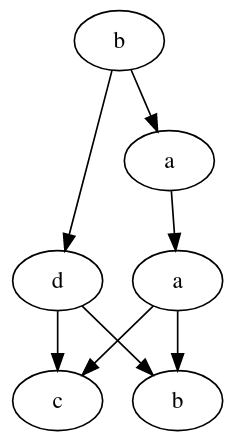
\includegraphics[width=3.5cm]{Screenshot_20231217_011732.png}\]

    \hypertarget{zadanie-2a}{%
\subsection{Zadanie 2a}\label{zadanie-2a}}

\begin{itemize}
\tightlist
\item
  \(I = \{(a, d), (d, a), (b, e), (e, b), (c, d), (d, c), (c, f), (f, c)\}\)
\item
  \(D = \bar{I}\)
\end{itemize}

Gdzie \(I\) - zbiór niezaleznych akcji, \(D\) - zbiór zależnych akcji.

    \hypertarget{zadanie-2b}{%
\subsection{Zadanie 2b}\label{zadanie-2b}}

    \hypertarget{fnf}{%
\subsubsection{FNF}\label{fnf}}

\begin{verbatim}
   a  b  c  d  e  f
0  *  b  *  *  e  *
1  *  b  *  *  *  *
2  *  *  *  *  *  *
3  *  *  c  *  *  f
4  *  *  c  d  *  *
5  *  *  *     *  *
6  a  *            
\end{verbatim}

\begin{itemize}
\tightlist
\item
  Popped top:
  \texttt{{[}\textquotesingle{}a\textquotesingle{},\ \textquotesingle{}d\textquotesingle{}{]}}
\item
  Removed markers:
  \texttt{{[}\textquotesingle{}b\textquotesingle{},\ \textquotesingle{}b\textquotesingle{},\ \textquotesingle{}c\textquotesingle{},\ \textquotesingle{}e\textquotesingle{},\ \textquotesingle{}e\textquotesingle{},\ \textquotesingle{}f\textquotesingle{},\ \textquotesingle{}f\textquotesingle{}{]}}
\end{itemize}

\begin{verbatim}
   a  b  c  d  e  f
0  *  b  *  *  e  *
1  *  b  *  *  *  *
2  *  *  *  *  *  *
3  *  *  c  *  *  f
4  *  *  c         
5  *               
\end{verbatim}

\begin{itemize}
\tightlist
\item
  Popped top:
  \texttt{{[}\textquotesingle{}c\textquotesingle{},\ \textquotesingle{}f\textquotesingle{}{]}}
\item
  Removed markers:
  \texttt{{[}\textquotesingle{}a\textquotesingle{},\ \textquotesingle{}a\textquotesingle{},\ \textquotesingle{}b\textquotesingle{},\ \textquotesingle{}b\textquotesingle{},\ \textquotesingle{}d\textquotesingle{},\ \textquotesingle{}e\textquotesingle{},\ \textquotesingle{}e\textquotesingle{}{]}}
\end{itemize}

\begin{verbatim}
   a  b  c  d  e  f
0  *  b  *  *  e  *
1  *  b  *  *  *  *
2  *  *  *  *     *
3  *     c         
\end{verbatim}

\begin{itemize}
\tightlist
\item
  Popped top: \texttt{{[}\textquotesingle{}c\textquotesingle{}{]}}
\item
  Removed markers:
  \texttt{{[}\textquotesingle{}a\textquotesingle{},\ \textquotesingle{}b\textquotesingle{},\ \textquotesingle{}e\textquotesingle{}{]}}
\end{itemize}

\begin{verbatim}
   a  b  c  d  e  f
0  *  b  *  *  e  *
1  *  b  *  *     *
2  *     *  *     *
\end{verbatim}

\begin{itemize}
\tightlist
\item
  Popped top:
  \texttt{{[}\textquotesingle{}b\textquotesingle{},\ \textquotesingle{}e\textquotesingle{}{]}}
\item
  Removed markers:
  \texttt{{[}\textquotesingle{}a\textquotesingle{},\ \textquotesingle{}a\textquotesingle{},\ \textquotesingle{}c\textquotesingle{},\ \textquotesingle{}c\textquotesingle{},\ \textquotesingle{}d\textquotesingle{},\ \textquotesingle{}d\textquotesingle{},\ \textquotesingle{}f\textquotesingle{},\ \textquotesingle{}f\textquotesingle{}{]}}
\end{itemize}

\begin{verbatim}
   a  b  c  d  e  f
0  *  b  *  *     *
\end{verbatim}

\begin{itemize}
\tightlist
\item
  Popped top: \texttt{{[}\textquotesingle{}b\textquotesingle{}{]}}
\item
  Removed markers:
  \texttt{{[}\textquotesingle{}a\textquotesingle{},\ \textquotesingle{}c\textquotesingle{},\ \textquotesingle{}d\textquotesingle{},\ \textquotesingle{}f\textquotesingle{}{]}}
\end{itemize}

\(FNF = (ad)(cf)(c)(be)(b)\)

    \hypertarget{lnf}{%
\subsection{LNF}\label{lnf}}

\begin{verbatim}
   a  b  c  d  e  f
0  *  b  *  *  e  *
1  *  b  *  *  *  *
2  *  *  *  *  *  *
3  *  *  c  *  *  f
4  *  *  c  d  *  *
5  *  *  *     *  *
6  a  *            
\end{verbatim}

\begin{itemize}
\tightlist
\item
  Popped action: \texttt{a}
\item
  Removed markers:
  \texttt{{[}\textquotesingle{}b\textquotesingle{},\ \textquotesingle{}c\textquotesingle{},\ \textquotesingle{}e\textquotesingle{},\ \textquotesingle{}f\textquotesingle{}{]}}
\end{itemize}

\begin{verbatim}
   a  b  c  d  e  f
0  *  b  *  *  e  *
1  *  b  *  *  *  *
2  *  *  *  *  *  *
3  *  *  c  *  *  f
4  *  *  c  d  *  *
5  *  *            
\end{verbatim}

\begin{itemize}
\tightlist
\item
  Popped action: \texttt{c}
\item
  Removed markers:
  \texttt{{[}\textquotesingle{}a\textquotesingle{},\ \textquotesingle{}b\textquotesingle{},\ \textquotesingle{}e\textquotesingle{}{]}}
\end{itemize}

\begin{verbatim}
   a  b  c  d  e  f
0  *  b  *  *  e  *
1  *  b  *  *  *  *
2  *  *  *  *  *  *
3  *  *  c  *  *  f
4  *  *     d     *
\end{verbatim}

\begin{itemize}
\tightlist
\item
  Popped action: \texttt{c}
\item
  Removed markers:
  \texttt{{[}\textquotesingle{}a\textquotesingle{},\ \textquotesingle{}b\textquotesingle{},\ \textquotesingle{}e\textquotesingle{}{]}}
\end{itemize}

\begin{verbatim}
   a  b  c  d  e  f
0  *  b  *  *  e  *
1  *  b  *  *  *  *
2  *  *  *  *  *  *
3  *  *     *     f
4           d     *
\end{verbatim}

\begin{itemize}
\tightlist
\item
  Popped action: \texttt{d}
\item
  Removed markers:
  \texttt{{[}\textquotesingle{}b\textquotesingle{},\ \textquotesingle{}e\textquotesingle{},\ \textquotesingle{}f\textquotesingle{}{]}}
\end{itemize}

\begin{verbatim}
   a  b  c  d  e  f
0  *  b  *  *  e  *
1  *  b  *  *  *  *
2  *  *  *  *     *
3  *        *     f
\end{verbatim}

\begin{itemize}
\tightlist
\item
  Popped action: \texttt{f}
\item
  Removed markers:
  \texttt{{[}\textquotesingle{}a\textquotesingle{},\ \textquotesingle{}b\textquotesingle{},\ \textquotesingle{}d\textquotesingle{},\ \textquotesingle{}e\textquotesingle{}{]}}
\end{itemize}

\begin{verbatim}
   a  b  c  d  e  f
0  *  b  *  *  e  *
1  *  b  *  *     *
2  *     *  *     *
\end{verbatim}

\begin{itemize}
\tightlist
\item
  Popped action: \texttt{b}
\item
  Removed markers:
  \texttt{{[}\textquotesingle{}a\textquotesingle{},\ \textquotesingle{}c\textquotesingle{},\ \textquotesingle{}d\textquotesingle{},\ \textquotesingle{}f\textquotesingle{}{]}}
\end{itemize}

\begin{verbatim}
   a  b  c  d  e  f
0  *  b  *  *  e  *
1  *     *  *     *
\end{verbatim}

\begin{itemize}
\tightlist
\item
  Popped action: \texttt{b}
\item
  Removed markers:
  \texttt{{[}\textquotesingle{}a\textquotesingle{},\ \textquotesingle{}c\textquotesingle{},\ \textquotesingle{}d\textquotesingle{},\ \textquotesingle{}f\textquotesingle{}{]}}
\end{itemize}

\begin{verbatim}
   a  b  c  d  e  f
0  *     *  *  e  *
\end{verbatim}

\begin{itemize}
\tightlist
\item
  Popped action: \texttt{e}
\item
  Removed markers:
  \texttt{{[}\textquotesingle{}a\textquotesingle{},\ \textquotesingle{}c\textquotesingle{},\ \textquotesingle{}d\textquotesingle{},\ \textquotesingle{}f\textquotesingle{}{]}}
\end{itemize}

\(LNF = accdfbbe\)

    \hypertarget{zadanie-2c}{%
\subsection{Zadanie 2c}\label{zadanie-2c}}

Korzystając z algorytmów, zaimplementowanych podczas wykonania
laboratorium 11, został wygenerowany następujący graf:

\begin{verbatim}
digraph g {
    1 -> 2
    1 -> 5
    2 -> 4
    3 -> 5
    4 -> 6
    4 -> 8
    5 -> 6
    5 -> 8
    6 -> 7
    1[label=a]
    2[label=c]
    3[label=d]
    4[label=c]
    5[label=f]
    6[label=b]
    7[label=b]
    8[label=e]
}
\end{verbatim}

który wygląda w sposób następujący:

\[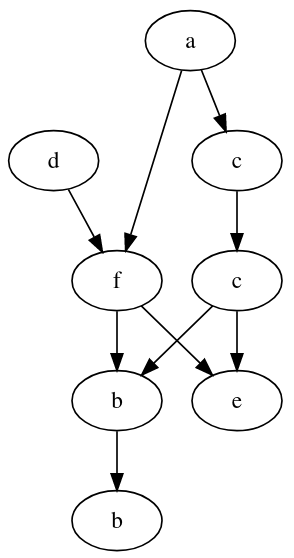
\includegraphics[width=4.5cm]{Screenshot_20231217_011857.png}\]

    \hypertarget{wnioski}{%
\section{Wnioski}\label{wnioski}}

\begin{itemize}
\item
  \textbf{Algorytm LNF} pozwala na wyznaczenie leksykograficznej postaci
  normalnej dowolnego słowa nad danym alfabetem względem danej relacji
  niezależności.
\item
  \textbf{Algorytm LNF} opiera się na zasadzie wyboru najmniejszej
  litery spośród dostępnych na stosach i usuwaniu znaczników z liter,
  które z nią nie komutują.
\item
  \textbf{Algorytm FNF} pozwala na wyznaczenie postaci normalnej Foaty
  dowolnego słowa nad danym alfabetem względem danej relacji
  niezależności.
\item
  \textbf{Algorytm FNF} opiera się na zasadzie tworzenia zbiorów liter z
  wierzchu stosów i uporządkowywania ich w kolejności alfabetycznej.
\item
  \textbf{Relacja niezależności} \(I\) jest relacją dwuargumentową,
  która określa, które litery w danym alfabecie mogą być zamienione
  miejscami bez zmiany znaczenia słowa.
\item
  \textbf{Relacja zależności} \(D\) to zbiór par liter, które nie można
  zamienić miejscami bez zmiany znaczenia słowa.
\item
  \textbf{Ślad} \([w]\) słowa \(w\) nad danym alfabetem względem danej
  relacji niezależności to zbiór wszystkich słów, które można otrzymać z
  \(w\) przez zamianę liter niezależnych.
\item
  \textbf{Graf zależności Diekerta} dla słowa \(w\) to graf skierowany,
  w którym wierzchołki odpowiadają literom słowa ww, a krawędzie
  odpowiadają relacji zależności \(D\).
\item
  \textbf{Graf zależności Diekerta} jest zminimalizowany, jeśli nie
  zawiera krawędzi ``przechodnich'', czyli takich, które można usunąć
  bez zmiany struktury grafu.
\end{itemize}

    \hypertarget{bibliografia}{%
\section{Bibliografia}\label{bibliografia}}

\begin{enumerate}
\def\labelenumi{\arabic{enumi}.}
\item
  Materiały do laboratorium 10, dr inż. Włodzimierz Funika:\\
  \url{https://home.agh.edu.pl/~funika/tw/lab-trace/}
\item
  Materiały do laboratorium 11, dr inż. Włodzimierz Funika:\\
  \url{https://home.agh.edu.pl/~funika/tw/lab-trace2/}
\item
  Trace Theory, Volker Diekert, Anca Muscholl:\\
  \url{http://www2.informatik.uni-stuttgart.de/fmi/ti/veroeffentlichungen/pdffiles/DiekertMuscholl2011.pdf}
\item
  Partial Commutation and Traces, Volker Diekert, Yves Métivier:\\
  \url{https://www.researchgate.net/publication/280851316_Partial_Commutation_and_Traces}
\item
  A Foata Normal Form And Its Application For The Purpose Of
  Accel­erating Computations By A Multi-GPU, Ahmet A. Husainov:\\
  \url{https://www.researchgate.net/publication/283389280_A_FOATA_NORMAL_FORM_AND_ITS_APPLICATION_FOR_THE_PURPOSE_OF_ACCEL-ERATING_COMPUTATIONS_BY_A_MULTI-GPU}
\end{enumerate}


    % Add a bibliography block to the postdoc
    
    
    
\end{document}
